\chapter{Representation of spacetime}
\section{Spacetime diagrams}
Now we will discuss the representation of spacetime with diagrams. Let's start from some basic concepts.\\
In a spacetime diagram an object that stays at rest is just an object with fixed spatial coordinates at any given time. This defines what is called a \textbf{world line}:
\begin{figure}[H]
  \centering
  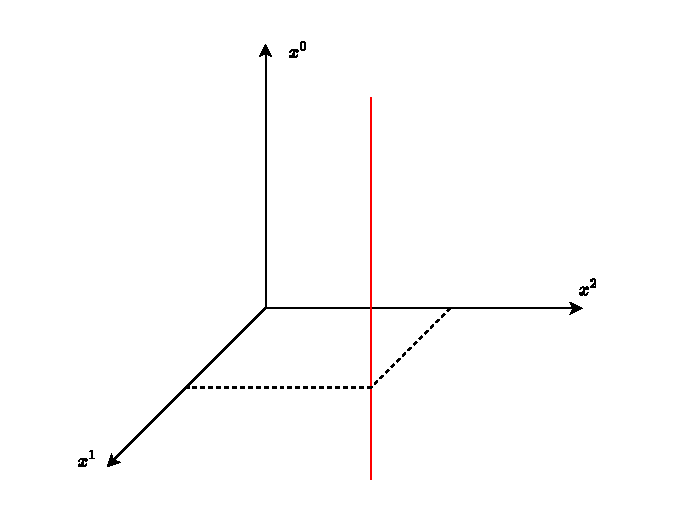
\includegraphics[width=0.8\linewidth]{res/svg/World_line.drawio}
\end{figure}
Instead an object moving in space has a space trajectory, which is the projection of the spacetime path onto the spatial coordinates, instead it must always increase in the time direction, giving a diagram of this type:
\begin{figure}[H]
  \centering
  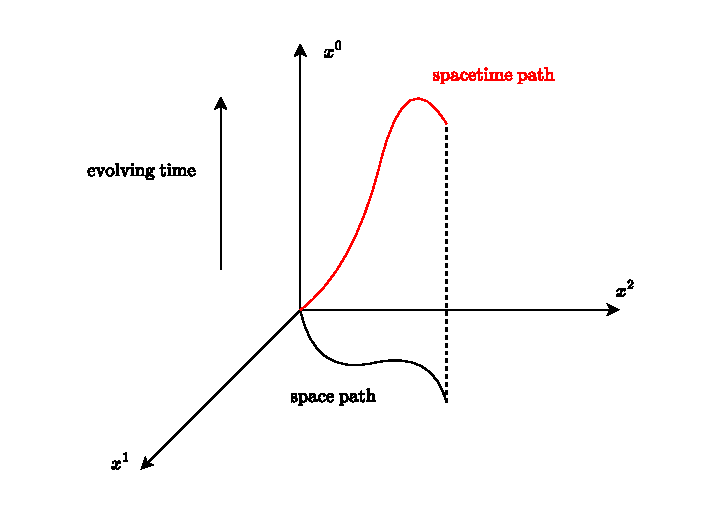
\includegraphics[width=0.8\linewidth]{res/svg/spacetime_path.drawio}
\end{figure}
Now we need to focus our attention on the limitations on the possible timepaths. For an infinitesimal displacement in space the object travels with velocity $u$ which must be lower then $c$, this means that the angle of the line tangent to the path is limited. We can represent the situation as:
\begin{figure}[H]
  \centering
  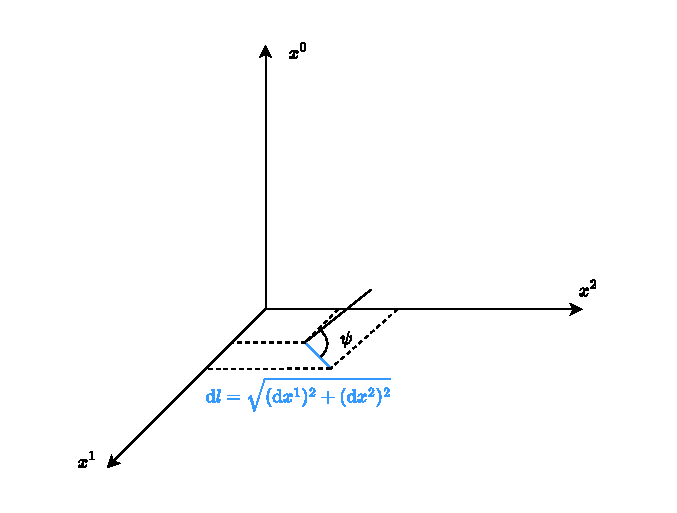
\includegraphics[width=0.8\linewidth]{res/svg/spacetime_angle.drawio}
\end{figure}
The tangent of $\psi$ is:
\begin{equation}
  \tan \psi = \dfrac{u}{c}
\end{equation}
For an object with mass this quantity is obviously limited by $1$ and so:
\begin{equation}
  \tan \psi < 1 \implies \psi < \qty{45}{\degree}
\end{equation}
And so any spacetime path of an object with mass is limited by a maximum angle of the tangent line equal to $\qty{45}{\degree}$. This identifies a well known geometric shape in the spacetime diagram which is called \textbf{light cone}:
\begin{figure}[H]
  \centering
  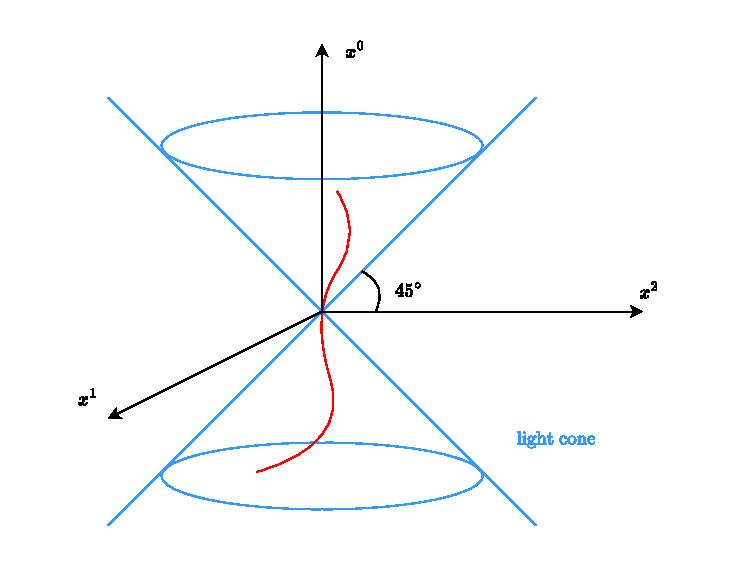
\includegraphics[width=0.8\linewidth]{res/svg/light_cone.drawio}
\end{figure}
Instead if we look at the spacetime path of a light beam it must be on the surface of the cone.\\
The light cone also divides spacetime in different regions.
\section{Events}
\subsection{Time-like events}
An event inside the cone must be such that:
\begin{equation} \label{e:timelike_condition}
  \norm{\Delta \vec{r}} < \Delta x^0
\end{equation}
But $\Delta x^0 = c\Delta t$ which means that:
\begin{equation}
  \dfrac{\norm{\Delta \vec{r}}}{\Delta t} < c
\end{equation}
So this event is in the \textbf{future} for the IRF. Equation \eqref{e:timelike_condition} also leads to:
\begin{equation}
  \Delta s^2 = \Delta x^0 - \norm{\Delta \vec{r}} > 0
\end{equation}
An event with $\Delta s^2 > 0$ is called \textbf{time-like}. If $\Delta x^0 < 0$ but $\norm{\Delta \vec{r}} < \abs{\Delta x^0}$ the event is still time-like, but it is in the past for the IRF.
\subsection{Space-like events}
Similarly, an event outside the cone is such that:
\begin{equation} \label{e:spacelike_condition}
  \norm{\Delta \vec{r}} > \Delta x^0
\end{equation}
But $\Delta x^0 = c\Delta t$ which means that:
\begin{equation}
  \norm{\Delta \vec{r}} > c\Delta t
\end{equation}
So there is no way a signal from the origin could travel fast enough to reach the point where the event will happen. This means that the event cannot be caused by something in the origin. This was also the condition necessary in order to be able to find a moving IRF such that the time order of the event is swapped.
In general an event with these properties satisfies:
\begin{equation}
  \Delta s^2 = \Delta x^0 - \norm{\Delta \vec{r}} < 0
\end{equation}
And is called \textbf{space-like event}.\\
The region outside the cone is called \textbf{undetermined present}.\\
